\section{Joint Distributions}

\subsection{Discrete Case}

Let $X,Y$ be discrete random variables, the function

\[ p_{XY}(x,y)=P(X=x,Y=y) \]

is called the joint PMF of $X$ and $Y$. \\

Joint PMFs share many properties with ordinary PMFs. For example, the total probability is one:

\[ \sum_i \sum_j p_{XY}(x_i,y_i) = 1 \]

To calculate the probability that $X$ takes values in range $[x_1, x_2]$ and $Y$ takes values in range $[y_1, y_2]$:

\[ P((x_1\le X\le x_2) \cap (y_1\le Y\le y_2)) = \sum_{x=x_1}^{x_2} \sum_{y=y_1}^{y_2} p_{XY}(x,y) \]

We can obtain PMF for $X$ alone from the joint PMF. It is called the marginal PMF of $X$ and is defined as

\[\ p_X(x)=P(X=x)=\sum_j p_{XY}(x,y_j) \]

Similarly for $Y$,

\[\ p_Y(y)=P(Y=y)=\sum_i p_{XY}(x_i,y) \]

The below shows an example joint PMF:

\begin{center}
	\begin{tabular}{|c|c|c|c|c|}
		\hline
		\diagbox{$Y$}{$X$} & $1$ & $2$ & $3$ & \\
		\hline
		$1$ & $1/4$ & $1/8$ & $1/8$ & $1/2$ \\
		\hline
		$4$ & $1/6$ & $1/3$ & $0$ & $1/2$ \\
		\hline
		& $10/24$ & $11/24$ & $3/24$ & \diagbox{$p_X$}{$p_Y$} \\
		\hline
	\end{tabular}
\end{center}

All of its entries sum up to one:

\[\frac14+\frac18+\frac18+\frac16+\frac13+0=1\]

Also, notice the total for $p_X$ and $p_Y$ add up to one as well.

\begin{texample}
	You toss $4$ dice. Let random variables $X$ denote the number of distinct results and $Y$ denote the minimal result. Find $P(X=1,Y=3)$ and $P(X=4,Y=3)$. \\
	
	$$P(1,3)=P(\{3, 3, 3, 3, 3\})=\frac{1}{6^4}$$
	
	$$P(4, 3)=P(\text{roll $3,4,5,6$ in some order})=\frac{4!}{6^4}$$
\end{texample}

\subsection{Continuous Case}

Let $X,Y$ be continuous random variables, the function $f_{XY}(x,y)$ is called the joint PDF of $X$ and $Y$. The probability can be calculated as follows

\[ P((X,Y)\in A) = \iint_A f_{XY}(x,y) dx \:dy \]

\begin{figure}[H]
	\centering
	\includegraphics[width=100mm]{21.png}
	\caption{Illustration of $A$}
\end{figure}

Joint PDFs share many properties with ordinary PDFs. For example, $f_{XY}(x,y)\ge0$ everywhere and

\[ \int_{-\infty}^\infty \int_{-\infty}^\infty f_{XY}(x,y) dx \:dy = 1 \]

To find the probability that $X$ takes values in range $[x_1, x_2]$ and $Y$ takes values in range $[y_1, y_2]$:

\[ P((x_1\le X\le x_2) \cap (y_1\le Y\le y_2)) = \int_{y_1}^{y_2} \int_{x_1}^{x_2} f_{XY}(x,y) dx \:dy \]

Marginal PDF for $X$:

\[ f_X(x)=\int_{-\infty}^\infty f(x,y) dy \]

Marginal PDF for $Y$:

\[ f_Y(y)=\int_{-\infty}^\infty f(x,y) dx \]

\begin{texample}
	Consider the following joint PDF:
	
	\[ f_{XY}(x,y)=\begin{cases} x+y & 0\le x,y \le1 \\ 0 & \text{otherwise} \end{cases} \]
	
	\begin{center}
		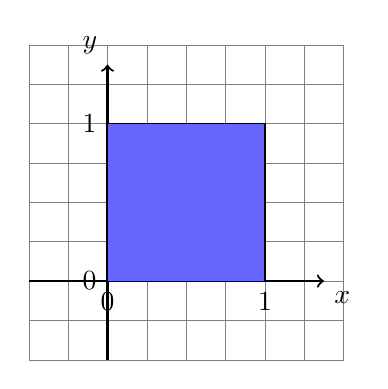
\begin{tikzpicture}[scale=0.5]
			\draw[step=1cm,gray,very thin] (-2,-2) grid (6,6);
			\draw[thick,->] (-2,0) -- (5.5,0) node[anchor=north west] {$x$};
			\draw[thick,->] (0,-2) -- (0,5.5) node[anchor=south east] {$y$};
			\foreach \x [count=\i from 0] in {0,4}
			\draw (\x cm,1pt) -- (\x cm,-1pt) node[anchor=north] {$\i$};
			\foreach \y [count=\i from 0] in {0,4}
			\draw (1pt,\y cm) -- (-1pt,\y cm) node[anchor=east] {$\i$};
			\filldraw[fill=blue!60!white, draw=black] (0,0) rectangle (4,4);
		\end{tikzpicture}
	\end{center}
	
	Find the marginal PDF for $X$. \\
	
	\[ f_X(x)=\int_{-\infty}^\infty f_{XY}(x,y) dy = \int_0^1 x+y\:dy = x+\frac12 \]
	
	\begin{center}
		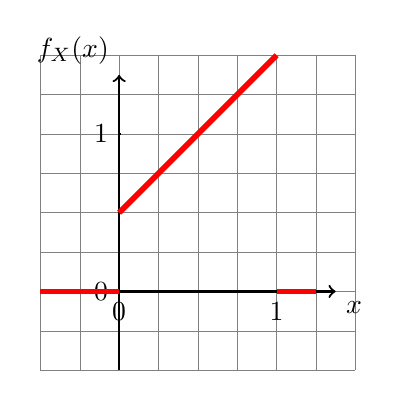
\begin{tikzpicture}[scale=0.5]
			\draw[step=1cm,gray,very thin] (-2,-2) grid (6,6);
			\draw[thick,->] (-2,0) -- (5.5,0) node[anchor=north west] {$x$};
			\draw[thick,->] (0,-2) -- (0,5.5) node[anchor=south east] {$f_X(x)$};
			\foreach \x [count=\i from 0] in {0,4}
			\draw (\x cm,1pt) -- (\x cm,-1pt) node[anchor=north] {$\i$};
			\foreach \y [count=\i from 0] in {0,4}
			\draw (1pt,\y cm) -- (-1pt,\y cm) node[anchor=east] {$\i$};
			\draw[line width=2pt,red] (-2,0) -- (0,0);
			\draw[line width=2pt,red] (4,0) -- (5,0);
			\draw[line width=2pt,red] (0,2) -- (4,6);
		\end{tikzpicture}
	\end{center}
\end{texample}

\subsection{Expectation}

If $X$ and $Y$ are random variables and $g$ is a function that takes these random variables, the expectation of $g(X,Y)$ is

\[ Eg(X,Y)=\sum_i \sum_j g(x_i,y_i)p(x_i,y_i) \]

for discrete random variables or

\[ Eg(x,y)=\int_{-\infty}^\infty \int_{-\infty}^\infty g(x,y)f(x,y) dx\:dy \]

for continuous random variables. For example, if $g(X,Y)=X+Y$, when $X$ and $Y$ are continuous,

\begin{align*}
	E[X+Y]&=\int_{-\infty}^\infty \int_{-\infty}^\infty (x+y)f(x,y) dx\:dy\\
	&=\int_{-\infty}^\infty \int_{-\infty}^\infty xf(x,y) dx\:dy+\int_{-\infty}^\infty \int_{-\infty}^\infty yf(x,y) dx\:dy\\
	&=EX+EY
\end{align*}

It turns out that the linearity of expectation still holds for multiple random variables:

\[E\left(\sum_i a_i X_i \right) = \sum_i a_i E(X_i)\]

\subsection{Independence}

The random variables $X$ and $Y$ are independent if for any $a,b \in \mathbb{R}$,

\[ P(X\le a, Y\le b)=P(X\le a) P(Y\le b) \]

ie. events $X\le a$ and $Y\le b$ are independent. In terms of PMF and PDF, $X$ and $Y$ are independent if

\[p_{XY}(x,y)=p_X(x)p_Y(y)\]

for discrete case and

\[f_{XY}(x,y)=f_X(x)f_Y(y)\]

for continuous case. \\

For any functions $g(X)$ and $h(Y)$, there exists a simple formula for calculating $E[g(X)h(Y)]$ when $X$ and $Y$ are independent.

\begin{align*}
	E[g(X)h(Y)]&=\int_{-\infty}^\infty \int_{-\infty}^\infty g(x)h(y) f(x,y) dx\: dy
	\intertext{Since $X$ and $Y$ are independent, $f(x,y)=f_X(x)f_Y(y)$,}
	&=\int_{-\infty}^\infty \int_{-\infty}^\infty g(x)h(y) f_X(x)f_Y(y) dx\: dy \\
	&=\left( \int_{-\infty}^\infty g(x) f_X(x) dx \right) \left( \int_{-\infty}^\infty h(y) f_Y(y) dy \right) \\
	&=E[g(X)]E[h(Y)]
\end{align*}

In particular, $E[XY]=E[X]E[Y]$. This works for discrete random variables as well.

\begin{texample}
	Consider the following joint PMF
	
	\[ p_{XY}(x,y)=\frac{x^2y}{30} \]
	
	for discrete random variables $X=1,2$ and $Y=1,2,3$. Show that $X$ and $Y$ are independent. \\
	
	The marginal PMF for $X$ is
	
	\[p_X(x)=\sum_{y=1}^3 \frac{x^2y}{30} = \frac{x^2}{5}\]
	
	The marginal PMF for $Y$ is
	
	\[p_Y(y)=\sum_{x=1}^2 \frac{x^2y}{30} = \frac{y}{6}\]
	
	Since
	
	\[p_{XY}(x,y)=p_X(x)p_Y(y)=\frac{x^2y}{30}\]
	
	So $X$ and $Y$ are independent.
\end{texample}

\begin{texample}
	The time $T$ (in hours past noon) until the arrival of the first taxi has $\Exp(6)$ distribution, and the time $B$ until first bus is independent with $\Exp(4)$ distribution. What is the joint probability density function of $T$ and $B$? Find the probability that the first taxi arrives before the first bus. If you arrive at noon and take the first bus or taxi (whichever arrives first), what is the distribution of your waiting time? \\
	
	The joint PDF for $T$ and $B$ is:
	
	\[ f_{TB}(t,b)=f_T(t)f_B(b)=\begin{cases} 6e^{-6t}4e^{-4t} & t,b \ge 0 \\ 0 & \text{otherwise} \end{cases} \]
	
	The probability that the first taxi arrives before the first bus $T<B$ is:
	
	\[P(T<B)=\iint_{t<b} f_{TB}(t,b)db\:dt=\int_0^\infty \int_t^\infty 6e^{-6t}4e^{-4t} db\:dt=\frac35\]
	
	To find the distribution for waiting time, denote a random variable $X = \min(T,B)$.
	
	\begin{align*}
		P(X>t)&=P(T>t,B>t)
		\intertext{Since $T$ and $B$ are independent,}
		&=P(T>t)P(B>t) \\
		&=\left(1-\int_0^t 6e^{-6t'} dt'\right)\left(1-\int_0^t 4e^{-4t'} dt'\right) \\
		&=\left(1-(1-e^{-6t})\right)\left(1-(1-e^{-4t})\right) \\
		&=e^{-6t}e^{-4t} \\
		&=e^{-10t}
	\end{align*}
	
	The CDF for $X$ is therefore
	
	\[P(X\le t)=1-P(X>t)=1-e^{-10t}\]
	
	It looks like the CDF for $\Exp(10)$.
\end{texample}

\begin{texample}
	If $X,Y$ are independent $\Norm(0,1)$ random variables, what is the distribution of $R=\sqrt{X^2+Y^2}$? \\
	
	The joint density is given by
	
	\[f_{XY})(x,y)=\frac{1}{2\pi}\exp\left(-\frac{x^2+y^2}{2}\right)\]
	
	We first calculate CDF for $R$:
	
	\begin{align*}
		F_R(a)&=P(\sqrt{X^2+Y^2}\le a) \\
		&=P(X^2+Y^2\le a^2) \\
		&=\iint_{x^2+y^2\le a^2} \frac{1}{2\pi}\exp\left(-\frac{x^2+y^2}{2}\right) dx\:dy
		\intertext{Changing to polar coordinates gives}
		&=\frac{1}{2\pi}\int_0^{2\pi} \int_0^a \exp\left(-\frac{r^2}{2}\right) r dr\:d\theta \\
		&=1-\exp\left(-\frac{a^2}{2}\right)
	\end{align*}
	
	PDF can be calculated via differentiating the CDF:
	
	\[f_R(a)=\frac{d}{da}\left( 1-\exp\left(-\frac{a^2}{2}\right) \right)=a\exp\left(-\frac{a^2}{2}\right)\]
\end{texample}

\begin{texample}
	A point $(X,Y)$ is uniformly chosen in the unit disc $x^2+y^2\leq 1$. (a) Determine the marginal PDF of $X$ and $Y$ and justify whether $X$ and $Y$ are independent. (b) Find the PDF of its distance from the origin $R = \sqrt{X^2+Y^2}$. Compute the expected distance from the origin. \\
	
	(a) The PDF for points uniformly distributed on the unit disk is given by:
	
	$$
	f_{XY}(x,y)=\begin{cases}
		c & x^2+y^2\leq 1 \\
		0 & \text{otherwise}
	\end{cases}
	$$
	
	The normalization factor $c$ is calculated by integrating over region $x^2+y^2\leq 1$ (this is same as finding the area of the unit circle):
	
	\[\iint_{x^2+y^2\leq 1} c dx\:dy = c\int_0^{2\pi}\int_0^1 rdr\:d\theta=c\pi=1 \]
	
	which gives $c=\frac{1}{\pi}$. \\
	
	The marginal PDFs for $X$ and $Y$ are:
	
	\[f_X(x)=\int_{-\sqrt{1-x^2}}^{\sqrt{1-x^2}} \frac{1}{\pi} dy = \frac{2}{\pi} \sqrt{1-x^2} \] for $x\in[-1,1]$.
	
	\[f_Y(y)=\int_{-\sqrt{1-y^2}}^{\sqrt{1-y^2}} \frac{1}{\pi} dx = \frac{2}{\pi} \sqrt{1-y^2} \] for $y\in[-1,1]$. \\
	
	Since $f_X(x)f_Y(y)\ne\frac{1}{\pi}$, $X$ and $Y$ are not independent. \\
	
	(b) The CDF for $R$ is:
	
	\[F_R(a)=P(X^2+Y^2\le a^2)=\iint_{x^2+y^2\leq a^2} f_{XY}(x,y) dx\:dy=\int_0^{2\pi}\int_0^a \frac{1}{\pi} rdr\:d\theta=a^2\]
	
	and its PDF is:
	
	\[f_R(a)=\frac{d}{da}(a^2)=2a\]
	
	So the expected distance from origin is given by:
	
	\[ER=\int_0^1 rf_R(r)dr=\int_0^1 2r^2dr=\frac23\]
\end{texample}

\begin{texample}
	Let $X,Y$ be uniform on the square $[0,2]\times[0,2]$. Find the distribution of the ratio $Z=X/Y$. \\
	
	We are given that
	
	\[f_{XY}(x,y)=\begin{cases} c & x\in[0,2]\:\text{and}\:y\in[0,2] \\ 0 & \text{otherwise} \end{cases}\]
	
	where $c$ is calculated by:
	
	\[\int_0^2\int_0^2 c dx\:dy=4c=1\]
	
	We first calculate the CDF for $Z$:
	
	\[F_Z(a)=P(Z\le a)=P\left(\frac{X}{Y}\le a\right)=P(X\le aY)\]
	
	To find $P(X\le aY)$, we need to consider two cases: $a\in[0,1]$ and $a\in[1,\infty)$.
	
	\begin{figure}[H]
		\centering
		\includegraphics[width=100mm]{34.png}
		\caption{Plot of the line $X=aY$ and integration regions in two cases.}
	\end{figure}
	
	For $a\in[0,1]$,
	
	\[P(X\le aY)=\int_0^2\int_0^{ay} \frac14 dx\:dy=\frac{a}{2}\]
	
	For $a\in[1,\infty)$,
	
	\[P(X\le aY)=1-\int_0^2\int_0^{\frac{x}{a}} \frac14 dy\:dx=1-\frac{1}{2a}\]
	
\end{texample}

\subsection{Covariance and Correlation Coefficient}

Covariance between two random variables $X$ and $Y$ is defined as

\[ \Cov(X,Y)=E[(X-EX)(Y-EY)] \]

In particular, $\Cov(X,X)=\Var(X)$. There is another formula for covariance:

\begin{align*}
	\Cov(X,Y)&=E[(X-EX)(Y-EY)] \\
	&=E[XY-(EX)Y-X(EY)+(EX)(EY)] \\
	&=E[XY]-E[X]E[Y]-E[X]E[Y]+E[X]E[Y] \\
	&=E[XY]-E[X]E[Y]
\end{align*}

\footnote{$\displaystyle E[XY]=\sum_i \sum_j x_iy_ip_{XY}(x_i,y_j)$} It follows that if $X$ and $Y$ are independent, $\Cov(X,Y)=0$ since $E[XY]=E[X]E[Y]$.

\begin{texample}
	Consider discrete random variables $X$ and $Y$, Their joint PMF is specified below
	
	\begin{center}
		\begin{tabular}{|c|c|c|}
			\hline
			\diagbox{$Y$}{$X$} & $0$ & $1$ \\
			\hline
			$-1$ & $0$ & $1/4$ \\
			\hline
			$1$ & $1/2$ & $1/4$ \\
			\hline
		\end{tabular}
	\end{center}
	
	Find $\Cov(X,Y)$. \\
	
	We have
	\[EX=0 \cdot \frac12 + 1 \cdot \left(\frac14+\frac14\right)=\frac12\]
	
	\[EY=-1\cdot \frac14+1\cdot\left(\frac12+\frac14\right)=\frac12\]
	
	\[E[XY]=-1\cdot\frac14+1\cdot\frac14=0\]
	
	Covariance of $X$ and $Y$ is therefore
	
	\[\Cov(X,Y)=E[XY]-EXEY=0-\frac12\cdot\frac12=-\frac14\]
	
\end{texample}

Covariance measures how much two random variables are \textit{linearly} related to each other (correlation). Positive covariance indicates that one variable is related to another variable linearly (e.g. when one variable is large, the other variable will also be large). The bigger the covariance is, the stronger the linear relationship becomes. Negative covariance indicates that there is an inverse linear relationship between two variables (eg. when one variable is small another variable will be big, and vice versa). When covariance is zero, $X$ and $Y$ do not have some linear relationship (ie. uncorrelated), but it does not necessarily imply that $X$ and $Y$ are independent. Again, consider continuous random variables $X \sim \Unif(-1,1)$ and $Y=X^2$. They are clearly dependent since $Y$ depends on the value of $X$\footnote{Note that you can't conclude that they are independent just because $E[XY]=E[X]E[Y]$. If $X$ and $Y$ are independent then $E[XY]=E[X]E[Y]$ but it is not necessarily true that if $E[XY]=E[X]E[Y]$ then $X$ and $Y$ are independent, only imply uncorrelateness.}.

\begin{texample}
	Show that $X$ and $Y$ are not independent. \\
	
	Independence means $P(X\le a, Y\le b)=P(X\le a) P(Y\le b)$ for any real numbers $a$ and $b$. Consider $a=\frac13$ and $b=\frac 14$. \\
	
	- $X \le \frac 13$, i.e. when $-1 \le X \le \frac13$, has probability $\frac{1+\frac13}{2}=\frac23$ \\
	- $Y \le \frac 14$, i.e. when $-\frac12 \le X \le \frac12$, has probability $\frac12$ \\
	- $X \le \frac 13, Y \le \frac 14$ together, i.e. when $-\frac12 \le X \le \frac13$, has probability $\frac5{12}$ \\
	
	but $\frac23 \times \frac12 \not=\frac5{12}$. This makes $X$ and $Y$ not independent.
\end{texample}

So, we have

$$E[X] = 0$$
$$E[Y] = E[X^2] = \int_{-1}^{1} x^2  dx = \frac23$$
$$E[XY] = E[X^3] = \int_{-1}^{1} x^3 dx = 0$$

The covariance is therefore

\[ \Cov(X,Y) = E[X^3] - E[X] E[X^2] = 0 - 0 \cdot \frac23 = 0 \]

This means $X$ and $Y$ do not depend on each other linearly.

\begin{figure}[H]
	\centering
	\includegraphics[width=100mm]{22.png}
	\caption{Sample of $1000$ points from the distribution. Points depend on each other quadratically but not linearly.}
\end{figure}

\begin{texample}
	Suppose $5$ cards are drawn from the standard deck of $52$ cards. Denote random variables $X$ to be the number of spades in the hand and $Y$ to be the number of black cards in the hand. Calculate $\Cov(X,Y)$. \\
	
	Let's try calculating $P(X=2,Y=4)$, the probability that a poker hand contains $4$ black cards and $2$ spades first. There are ${52 \choose 5}$ ways to choose $5$ cards from the deck, ${13\choose2}$ ways to select 2 spades, ${13\choose2}$ ways to select the remaining 2 black cards excluding spades, and ${26\choose1}$ ways to choose a red card. The probability is
	
	\[ P(X=2,Y=4)=\frac{{13\choose2}{13\choose2}{26\choose1}}{{52\choose5}} \]
	
	We can generalize this result to $x$ spades and $y$ black cards to create the joint PMF for $X$ and $Y$:
	
	\[ p_{XY}(x,y)=P(X=x,Y=y)=\frac{{13\choose x}{13\choose y-x}{26\choose 5-y}}{{52\choose5}} \]
	
	This gives nonzero probability when $X\le Y$. The joint PMF table is given below:
	
	\begin{center}
		\footnotesize
		\begin{tabular}{|c|c|c|c|c|c|c|c|}
			\hline
			\diagbox{$Y$}{$X$} &         $0$&         $1$&         $2$&         $3$&         $4$&         $5$& \\
			\hline
			$0$ & $0.025310$ & $0.000000$ & $0.000000$ & $0.000000$ & $0.000000$ & $0.000000$ & $0.02531$ \\
			\hline
			$1$ & $0.074780$ & $0.074780$ & $0.000000$ & $0.000000$ & $0.000000$ & $0.000000$ & $0.14956$ \\
			\hline
			$2$ & $0.078031$ & $0.169068$ & $0.078031$ & $0.000000$ & $0.000000$ & $0.000000$ & $0.32513$ \\
			\hline
			$3$ & $0.035764$ & $0.126801$ & $0.126801$ & $0.035764$ & $0.000000$ & $0.000000$ & $0.32513$ \\
			\hline
			$4$ & $0.007153$ & $0.037195$ & $0.060864$ & $0.037195$ & $0.007153$ & $0.000000$ & $0.14956$ \\
			\hline
			$5$ & $0.000495$ & $0.003576$ & $0.008583$ & $0.008583$ & $0.003576$ & $0.000495$ & $0.02531$ \\
			\hline
			& $0.221534$ & $0.411420$ & $0.274280$ & $0.081543$ & $0.010729$ & $0.000495$ & \diagbox{$p_X$}{$p_Y$} \\
			\hline
		\end{tabular}
	\end{center}
	
	With expectation values
	
	\[EX=1.25\]
	\[EY=2.5\]
	
	There are two ways to calculate covariance: use $E[(X-EX)(Y-EY)]$ or $E[XY]-E[X]E[Y]$. Both methods give the same answer:
	
	\[\Cov(X,Y)=\sum_{y=0}^5\sum_{x=0}^5 (x-EX)(y-EY) p_{XY}(x,y)=0.575980\]
	
	\[\Cov(X,Y)=\left( \sum_{y=0}^5\sum_{x=0}^5 xyp_{XY}(x,y) \right)-(EX)(EY)=0.575980\]
	
	When the number of spades increases, the number of black cards also increases. \\
	
	Most of the computations in this example are handled by Python\footnote{\href{https://gist.github.com/marethyu/777e372c69cb356c5fc8c93f59cf62e6}{Source code}}.
\end{texample}

Correlation coefficient $\rho(X,Y)$ of $X$ and $Y$ is defined as

\[\rho(X,Y)=\frac{\Cov(X,Y)}{\sqrt{\Var(X)\Var(Y)}}\]

It is a unitless quantity that measures correlation between $X$ and $Y$. It can be thought as the a normalized version of covariance since it takes values between $-1$ and $1$. To prove this statement, consider the following theorem:

\begin{theorem}
	Cauchy-Schwarz Inequality: $|E(XY)|^2 \le E(X^2)E(Y^2)$
\end{theorem}

\begin{proof}
	Define a new random variable $Z=X+\lambda Y$ where $\lambda$ is some real number. \\
	
	The expectation for $Z^2$ is
	
	\begin{align*}
		E(Z^2)&=E((X+\lambda Y)^2) \\
		&=E(X^2+2\lambda XY+\lambda^2Y^2) \\
		&=E(X^2)+2\lambda E(XY)+\lambda^2 E(Y^2)
	\end{align*}
	
	Clearly, $E(Z^2)$ cannot be less than 0: $E(Z^2)\ge0$. Let $c=E(X^2)$, $b=2E(XY)$ and $a=E(Y^2)$,
	
	\[ a\lambda^2+b\lambda+c\ge0 \]
	
	Recall that a quadratic equation that gives positive values for all $\lambda$ should have discriminant $b^2-4ac \le 0$. This means
	
	\[(2E(XY))^2-4E(X^2)E(Y^2)\le0\]
	\[E(XY)^2-E(X^2)E(Y^2)\le0\]
	
	We finally get the equality:
	
	\[|E(XY)|^2 \le E(X^2)E(Y^2)\]
	
\end{proof}

We will now apply this inequality to show that $\rho(X,Y)$ is normalized.

\begin{theorem}
	$\rho(X,Y)$ only takes values between $-1$ and $1$.
\end{theorem}

\begin{proof}
	We know that $\Cov(X,Y)=E[(X-EX)(Y-EY)]$. Applying the Cauchy-Schwarz inequality to $E[(X-EX)(Y-EX)]$ gives
	
	\[|E[(X-EX)(Y-EY)]|^2 \le E[(X-EX)^2]E[(Y-EY)^2]\]
	
	By the definition of variance,
	
	\[|\Cov(X,Y)|^2 \le \Var(X)\Var(Y)\]
	
	\[\frac{|\Cov(X,Y)|^2}{\Var(X)\Var(Y)} \le 1\]
	
	Taking square root gives
	
	\[|\rho| \le 1\]
	
	So $-1\le\rho\le1$.
\end{proof}

It can be shown that

\[\rho(X,Y)=\begin{cases} 1 & \text{iff $Y=aX+b$ where $a,b\in\mathbb{R}$ and $a>0$} \\ -1 & \text{iff $Y=aX+b$ where $a,b\in\mathbb{R}$ and $a<0$} \end{cases}\]

In other words, $|\rho|=1$ if there is a direct linear relationship between $X$ and $Y$.

\subsection{Variance and Independence}

\begin{theorem}
	If $X,Y$ are independent then
	
	\[\Var(X+Y)=\Var(X)+\Var(Y)\]
\end{theorem}

\begin{proof}
	\begin{align*}
		\Var(X+Y)&=E((X+Y)^2)-(E(X+Y))^2 \\
		&=E(X^2+2XY+Y^2)-(EX+EY)^2 \\
		&=E(X^2)+2E(XY)+E(Y^2)-((EX)^2+2(EX)(EY)+(EY)^2) \\
		&=(E(X^2)-(EX)^2)+(E(Y^2)-(EY)^2)+2(E(XY)-(EX)(EY)) \\
		&=\Var(X)+\Var(Y)+2\Cov(X,Y)
		\intertext{Since $X,Y$ are independent, $\Cov(X,Y)=0$,}
		&=\Var(X)+\Var(Y)
	\end{align*}
\end{proof}

This result can be generalized to multiple random variables:

\[\Var\left( \sum_i X_i \right) = \sum_i \Var(X_i)\]

\begin{texample}
	Find variance for a binomial random variable $X\sim\Bin(n,p)$. \\
	
	We can write $X$ in terms of $n$ independent Bernoulli trials:
	
	\[X=X_1+X_2+\cdots+X_n\]
	
	where $X_i$ are Bernoulli random variables. \\
	
	Since $X_i$s are independent from each other,
	
	\[\Var(X)=\Var\left( \sum_{i=1}^n X_i \right) = \sum_{i=1}^n \Var(X_i)\]
	
	For a single trial, the variance is
	
	\[\Var(X_i)=E(X_i^2)-(E(X_i))^2\]
	
	Since $X_i^2=X_i$ and expectation for Bernoulli random variable is $p$,
	
	\[\Var(X_i)=E(X_i)-(E(X_i))^2=p-p^2\]
	
	The variance for a binomial random variable is therefore
	
	\[\Var(X) = \sum_{i=1}^n p-p^2 = np(1-p)\]
\end{texample}

\subsection{Sum of Independent Random Variables}

Let $X$ and $Y$ be independent discrete random variables. The PMF of its sum $X+Y$ is:

\[p_{X+Y}(n)=P(X+Y=n)\]

To calculate $P(X+Y=n)$, we need to consider all possible combinations of $X$ and $Y$ that add up to $n$. This gives

\[p_{X+Y}(n)=\sum_{j=0}^n P(X=j,Y=n-j)=\sum_{j=0}^n P(X=j)P(Y=n-j)\]

where the last formula holds because $X$ and $Y$ are independent. The PMF $p_{X+Y}(n)$ is known as the convolution of PMFs $p_X(n)$ and $p_Y(n)$.

\begin{texample}
	Suppose $X$ and $Y$ are independent Poisson random variables with parameters $\lambda_1$ and $\lambda_2$ respectively. Find the PMF of $X+Y$. \\
	
	For $n=0,1,2,\dots$, we have
	
	\begin{align*}
		p_{X+Y}(n)&=\sum_{j=0}^n P(X=j)P(Y=n-j) \\
		&=\sum_{j=0}^n \frac{\lambda_1^j e^{-\lambda_1}}{j!} \frac{\lambda_2^{n-j}e^{-\lambda_2}}{(n-j)!} \\
		&=e^{-(\lambda_1+\lambda_2)} \frac{1}{n!} \sum_{j=0}^n {n \choose j} \lambda_1^j \lambda_2^{n-j}
		\intertext{Applying binomial theorem $(a+b)^n=\sum_{k=0}^n{n \choose k} a^k b^{n-k}$,}
		&=e^{-(\lambda_1+\lambda_2)} \frac{(\lambda_1+\lambda_2)^n}{n!}
	\end{align*}
	
	We got $X+Y \sim \Pois(\lambda_1+\lambda_2)$
\end{texample}

The calculation is similar to binomial random variables. Suppose $X\sim\Bin(n,p)$ and $Y\sim\Bin(m,p)$, then $X+Y\sim\Bin(n+m,p)$. \\

Now, suppose $X$ and $Y$ are continuous independent random variables. The CDF for $X+Y$ is:

\[F_{X+Y}(a)=P(X+Y\le a)=\iint_R f_X(x)f_Y(y) dx\:dy\]

where $R$ is the region that satisfied inequality $x+y\le a$.

\begin{figure}[H]
	\centering
	\includegraphics[width=100mm]{23.png}
	\caption{Illustration of the Inequality $x+y\le a$}
\end{figure}

\begin{align*}
	F_{X+Y}(a)&=\iint_R f_X(x)f_Y(y) dx\:dy \\
	&=\int_{-\infty}^\infty \left( \int_{-\infty}^{a-y} f_X(x) dx \right) f_Y(y) dy \\
	&=\int_{-\infty}^\infty F_X(a-y) f_Y(y) dy
\end{align*}

We found the convolution for $F_X(a)$ and $F_Y(a)$. To find PDF for $X+Y$, we differentiate $F_{X+Y}(a)$ which gives

\begin{align*}
	f_{X+Y}(a)&=\frac{d}{da} F_{X+Y}(a) \\
	&=\int_{-\infty}^\infty \left[ \frac{d}{da}F_X(a-y) \right] f_Y(y) dy \\
	&=\int_{-\infty}^\infty f_X(a-y) f_Y(y) dy
\end{align*}

\begin{texample}
	For $X\sim \Unif(0,a)$ and $Y\sim \Unif(0,b)$, calculate the probability density for $X+Y$, assuming that $a<b$. \\
	
	\begin{figure}[H]
		\centering
		\includegraphics[width=100mm]{24.png}
		\caption{Illustrations for PDFs $f_X(x)$, $f_Y(x)$ and $f_X(-x)$}
	\end{figure}
	
	The formula for finding convolution is:
	
	\[ f_{X+Y}(t)=\int_{-\infty}^\infty f_X(t-x) f_Y(x) dx \]
	
	We need to integrate the product $f_X(t-x)$ (which is basically the flipped version of $f_X(x)$) and $f_Y(x)$. Unfortunately, calculating the integral is not easy. We need to consider different cases for $t$. The ranges of $t$ that gives nonzero product are: $0<t<a$, $a<t<b$, and $b<t<a+b$. Integral is different in each case. \\
	
	Let's start with range $0<t<a$,
	
	\begin{figure}[H]
		\centering
		\includegraphics[width=100mm]{25.png}
	\end{figure}
	
	The product in this range is $\frac1a \frac1b = \frac{1}{ab}$ and the integral is
	
	\[f_{X+Y}(t)=\int_0^t \frac{1}{ab} dx = \frac{t}{ab}\]
	
	For range $a<t<b$,
	
	\begin{figure}[H]
		\centering
		\includegraphics[width=100mm]{26.png}
	\end{figure}
	
	\[f_{X+Y}(t)=\int_{t-a}^t \frac{1}{ab} dx = \frac{1}{b}\]
	
	Finally for range $b<t<a+b$,
	
	\begin{figure}[H]
		\centering
		\includegraphics[width=100mm]{27.png}
	\end{figure}
	
	\[f_{X+Y}(t)=\int_{t-a}^b \frac{1}{ab} dx = \frac{a+b-t}{ab}\]
	
	The final answer is:
	
	\[f_{X+Y}(t) = \begin{cases} \frac{t}{ab} & 0 < t < a \\ \frac1b & a < t < b \\ \frac{a+b-t}{ab} & b<t<a+b \\ 0 & \text{otherwise} \end{cases}\]
	
	The graph of this PDF looks like the following:
	
	\begin{figure}[H]
		\centering
		\includegraphics[width=100mm]{28.png}
	\end{figure}
	
	This PDF shows probable $t$ values that can be decomposed into the sum $X+Y$. It is peaked in range $[a,b]$ because there are many ways to obtain the values between $a$ and $b$ than other points. There is only one way to obtain either $0$ or $a+b$, so their probabilities are close to zero.
\end{texample}

\begin{texample}
	Busy server queue: A web server has $n$ pending tasks. Find a PDF for calculating total time it takes to complete all tasks. \\
	
	Denote a random variable $X_i$ to be the time taken for completing task $i$. They are assumed to be independent from each other and can be modelled with an exponential random variable with parameter $\lambda$. \\
	
	We start by calculating PDF for $X_1+X_2$, the time of completion of task $2$. Applying the convolution formula we derived:
	
	\begin{align*}
		f_{X_1+X_2}(x)&=\int_{-\infty}^\infty f_{X_1}(x-y) f_{X_2}(y) dy \\
		&=\int_0^x \lambda e^{-\lambda (x-y)} \lambda e^{-\lambda y} dy \\
		&=\lambda^2 e^{-\lambda x} \int_0^x dy \\
		&=\lambda^2 xe^{-\lambda x}
	\end{align*}
	
	The below plot compares two PDFs $f_{X_1}(x)$ and $f_{X_1+X_2}(x)$:
	
	\begin{figure}[H]
		\centering
		\includegraphics[width=100mm]{29.png}
		\caption{$f_{X_1}(x)$ and $f_{X_1+X_2}(x)$}
	\end{figure}
	
	It shows that the likely completion time for task $2$ is later than the completion time for task $1$. \\
	
	Next, we calculate PDF for $X_1+X_2+X_3$ which gives:
	
	\begin{align*}
		f_{X_1+X_2+X_3}(x)&=\int_{-\infty}^\infty f_{X_1+X_2}(x-y) f_{X_3}(y) dy \\
		&=\int_0^x \lambda^2 (x-y)e^{-\lambda (x-y)} \lambda e^{-\lambda y} dy \\
		&=\lambda^3 x^2\frac{e^{-\lambda x}}{2}
	\end{align*}
	
	and here is the comparison again:
	
	\begin{figure}[H]
		\centering
		\includegraphics[width=100mm]{30.png}
		\caption{$f_{X_1}(x)$, $f_{X_1+X_2}(x)$ and $f_{X_1+X_2+X^3}(x)$}
	\end{figure}
	
	We can generalize our PDF for $n$ tasks as follows:
	
	\[f_{X_1+X_2+\cdots+X_n}(x)=\lambda^nx^{n-1}\frac{e^{-\lambda x}}{(n-1)!}\]
	
	This is the distribution for Gamma random variable: $X_1+X_2+\cdots+X_n\sim\text{Gamma}(n,\lambda)$.
\end{texample}

\subsection{Teaser: Poisson Processes}

The busy server queue example we did is an example of Poisson process. Task completions occur continuously and independently. Denote random variable $N_t$ be the number of tasks completed by time $t$. The expectation for this random variable is:

\[E[N_t]=\lambda t\]

It makes sense because $\lambda$ can be interpreted as number of tasks done per unit time (ie. rate), so multiplying it by time $t$ will give the expected number of tasks done. \\

Let's find a PMF for $N_t$.  We start by calculating $P(N_t\ge n)$ which is equivalent to $P(X_1+X_2+\cdots+X_n\le t)$, the probability that $n$ tasks completed by time $t$.

\begin{align*}
	P(N_t\ge n)&=P(X_1+X_2+\cdots+X_n\le t) \\
	&=\int_0^t \frac{\lambda^nx^{n-1}}{(n-1)!} e^{-\lambda x} dx
	\intertext{Change of variables using $u=\lambda x$ gives,}
	&=\int_0^{\lambda t} \frac{u^{n-1}}{(n-1)!} e^{-u} du
	\intertext{Integration by parts gives,}
	&=-\left.\frac{u^{n-1}}{(n-1)!}e^{-u}\right\vert_0^{\lambda t} + \int_0^{\lambda t} \frac{u^{n-2}}{(n-2)!} e^{-u} du \\
	&=-\frac{(\lambda t)^{n-1}}{(n-1)!} e^{-\lambda t} + P(N_t \ge n - 1)
\end{align*}

Finally,

\[P(N_t=n-1)=P(N_t \ge n-1) - P(N_t \ge n) = \frac{(\lambda t)^{n-1}}{(n-1)!} e^{-\lambda t}\]

We conclude that $N_t$ is a Poisson random variable with parameter $\lambda t$: $N_t\sim\Pois(\lambda t)$.
